\documentclass[11pt]{article}

% Use the following to compile
% mkdir tmp
% pdflatex -aux-directory=tmp -output-directory=tmp --shell-escape notes.tex

% Package use definitions
\usepackage[margin=1in]{geometry}
\usepackage{fancyhdr}
\usepackage[parfill]{parskip}
\usepackage{graphicx}
\usepackage{comment}
\usepackage[outputdir=tmp]{minted}
\usepackage[dvipsnames]{xcolor}
\usepackage{listings}
\usepackage[hidelinks]{hyperref}
\usepackage{amsmath}
\usepackage{amsfonts}
\usepackage{amssymb}
\usepackage{tcolorbox}
\usepackage{tabu}
\usepackage{upgreek}
\usepackage[ruled,vlined]{algorithm2e}
\usepackage[nottoc]{tocbibind}
\usepackage{natbib}
\usepackage{pdfpages}
\usepackage{pgffor}

\setlength{\parindent}{11pt}
\setlength{\parskip}{0pt}

% Header and footer setup
\pagestyle{fancy} \rhead{\today} \lhead{Enquette Budget Temps} \renewcommand{\headrulewidth}{1pt} \renewcommand{\footrulewidth}{1pt}

% Image directory specification
\graphicspath{ {./images/} }

% Settings minted option for the entire document
\definecolor{LightGray}{rgb}{0.9, 0.9, 0.9}
\setminted{frame=lines,framesep=2mm,linenos,
  fontsize=\footnotesize, baselinestretch=1.2}

% Start of document
\begin{document}

% Title page and table of contents setup
\begin{titlepage}
  \begin{center}
    \vspace*{1cm} \Huge \textbf{Enquette Budget Temps}\\
    \vspace*{1\baselineskip} Langage R et Analyse de donnée\\
    \vspace*{2\baselineskip} \large
    \vfill \normalsize \textbf{Etienne Sharpin}\\ \textbf{Jose
      A. Henriquez Roa}\\
    \vspace*{2\baselineskip} \today \rhead{\today}
    \newpage
    \normalsize \tableofcontents
    \newpage
  \end{center}
\end{titlepage}
%% \section{Description du jeu de données}
%% \section{Chargement des données}
%% \section{Normalisation des distributions}
%% \section{Analyse des boîtes à moustaches}
%% \section{Matrice de corrélation}

%% \section{Clustering}
%% \section{comparaison des profils}

\section{Carte Radar}
For comparion of the time allocated to different tasks between individuals of
different groups we have choosen the method of radar chart. The following code
snippet shows how we plotted these charts for all 28 groups, shown in the
annex. Along with a radar chart containing all groups containing all groups
shown at the end of this section.
\begin{minted}{R}
library(fmsb)

pdf("plot/radar-chart-all.pdf")
df04 <- rbind(rep(max(df03),28), rep(min(df03),28), df03)
radarchart(df04, title="Per-Instance comparison")
dev.off()

for (i in 1:28) {
    pdf(paste("plot/radar-chart/radar-chart-", tolower(df01$ID[i]), ".pdf", sep=""))
    df05 <- rbind(rep(max(df03),28), rep(min(df03),28), df03[i,])
    radarchart(df05, title=df01$ID[i])
    dev.off()
}
\end{minted}
For this we have used the library \textit{fmsb} which includes the function
\textit{radarchart(...)} from which the plots were drawn. Figure
\ref{fig:radar-chart-all} shows a comparison of time distributions between all
groups present in the dataset. The individual radar charts can be found in the
annex \ref{section:annex}
\begin{figure}[h]
  \centering
  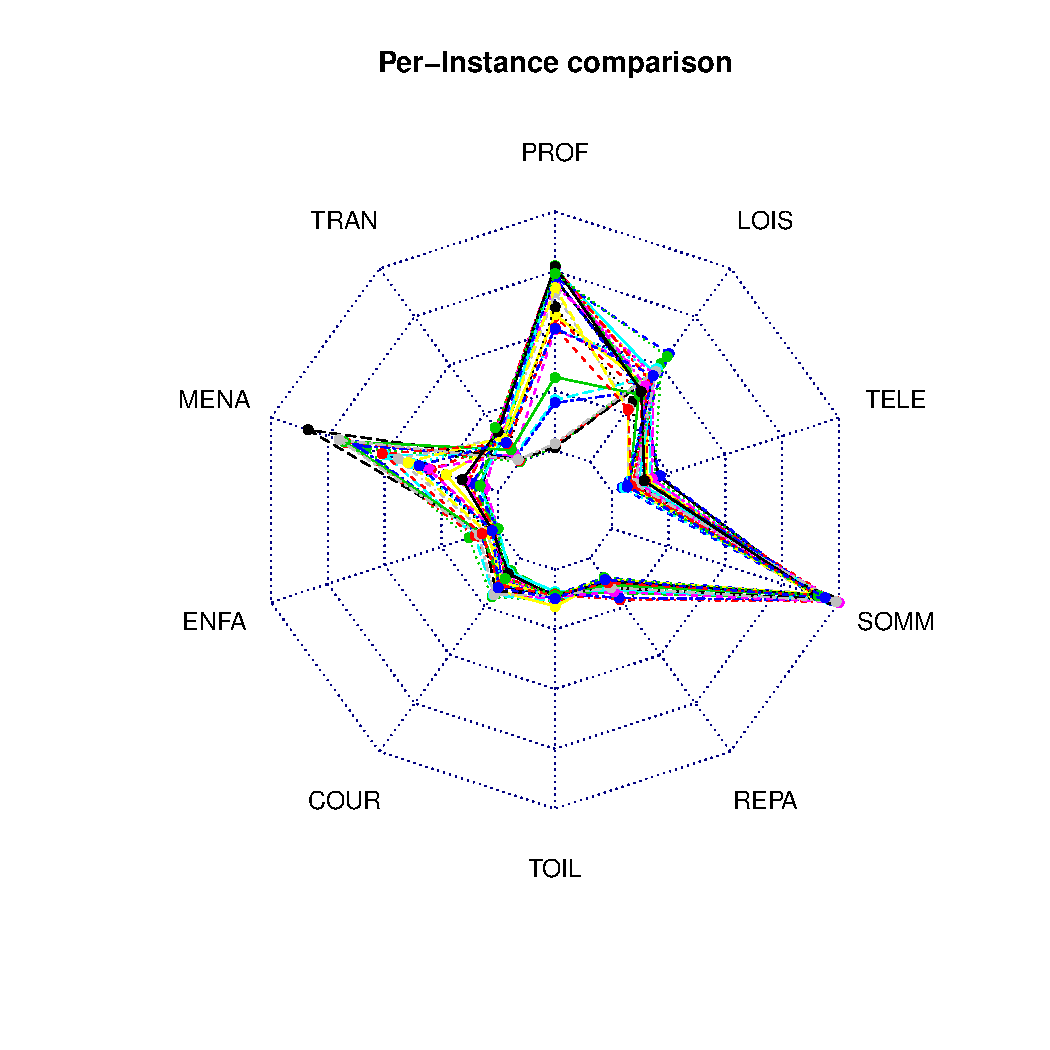
\includegraphics[scale=0.55]{../plot/radar-chart-all.pdf}
  \caption{Comparison in between all profile groups}
  \label{fig:radar-chart-all}
\end{figure}
\section{Graphique à barres}
Since, radar charts that incorporate reference values tend to look rather
clutered we have also chosen to visualize time distribution with the use of bar
plots, in which we have included the time percentages in the y axis.
\begin{minted}{R}
for (i in 1:28) {
    pdf(paste("plot/bar-plot/bar-plot-", tolower(df01$ID[i]), ".pdf", sep=""))
    barplot(t(as.matrix(df03[i,])), beside=TRUE, main=df01$ID[i],
            ylab="Time percentage", names.arg=colnames(df03), las=2)
    dev.off()
}
\end{minted}
The generated plots are in the annex \ref{section:annex}
\section{ACP}
The following line performs the PCA which we use in the following clustering
section for visualization of instance clustering results.
\begin{minted}{R}
  pca = prcomp(df03)
\end{minted}
The percentages of the explained variance for each principal component is gotten
through the following command.
\begin{minted}{R}
  summary(pca)$importance[2,]
\end{minted}
which produces the following output:\\\\ \texttt{PC1:\ 0.8804 PC2:\ 0.07166
  PC3:\ 0.02654 PC4:\ 0.01521 PC5:\ 0.0032 PC6:\ 0.00158 \\PC7:\ 0.00072
  PC8:\ 0.00043 PC9:\ 0.00026 PC10:\ 0}\\\\ As we can see a little more that
95\% of the variance is explained by the two first principal components. Which
means that the two dimensional projection of the data will be of fairly good
quality.\par The followng plots a graphical representation of the above output
\begin{minted}{R}
pdf("plot/principal-component-explained-variance.pdf")
barplot(summary(pca)$importance[2,],ylab="Explained Variance Proportion",
        ylim=c(0,1), main="Principal Component Explained Variance")
dev.off()   
\end{minted}
The resulting plot can be seen in figure
\ref{fig:principal-component-explained-variance}.\par
\begin{figure}[H]
  \centering
  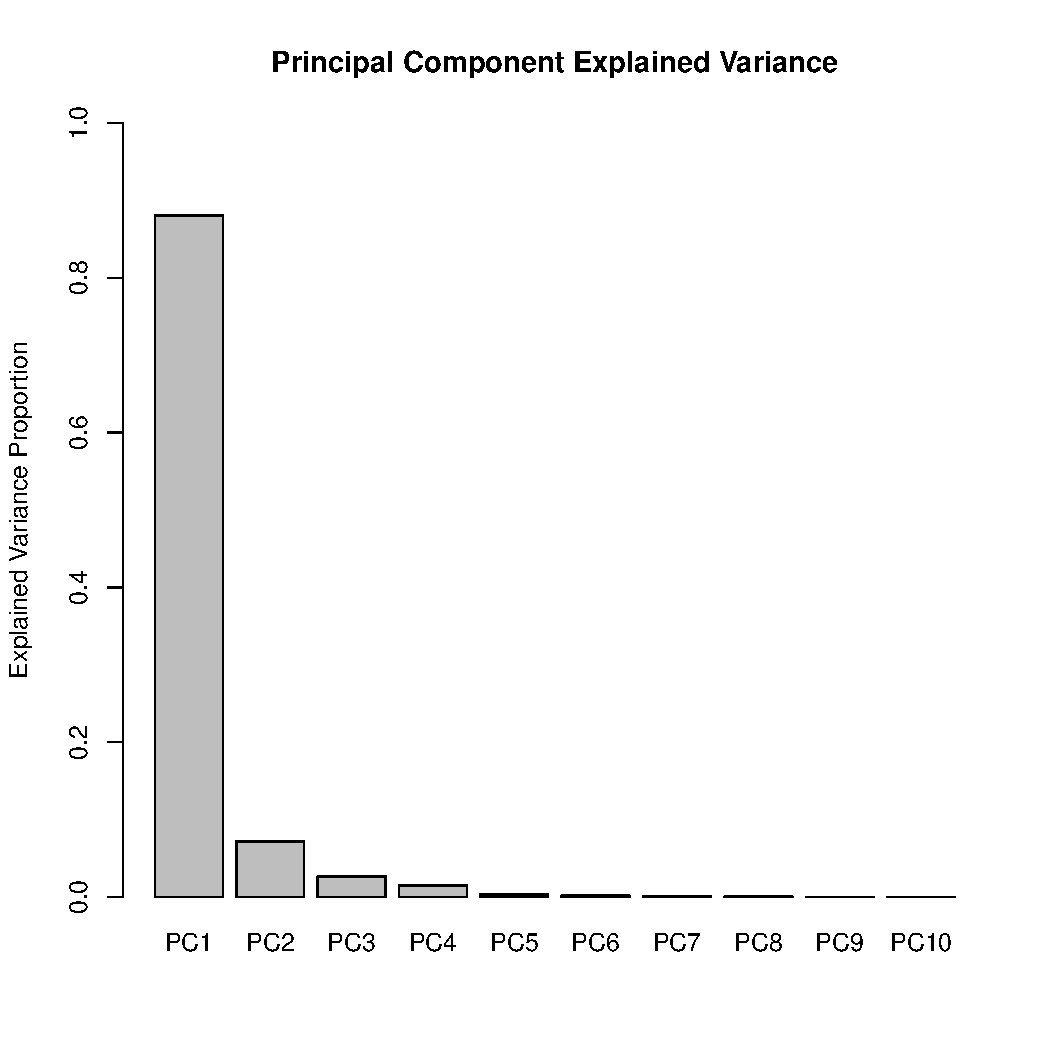
\includegraphics[scale=0.5]{../plot/principal-component-explained-variance.pdf}
  \caption{Principal component explained variance}
  \label{fig:principal-component-explained-variance}
\end{figure}
The following code snippet shows the projection of all attributes into the two
first principal components.
\begin{minted}{R}
pdf("plot/pca-attribute-projection.pdf")
library("factoextra")
fviz_pca_var(pca, col.var = "cos2", col.ind = "cos2",
             gradient.cols = c("#00AFBB", "#E7B800", "#FC4E07"))
dev.off()
\end{minted}
As show in figure \ref{fig:pca-attribute-projection}. In this one we see that
the two best projected attributes are by far the PROF and MENA attributes,
corresponding respectively to the attributes designating the time spent working
and cleaning.\par Next, the visualization of the instance projection was done
through the following code.
\begin{figure}[h]
  \centering
  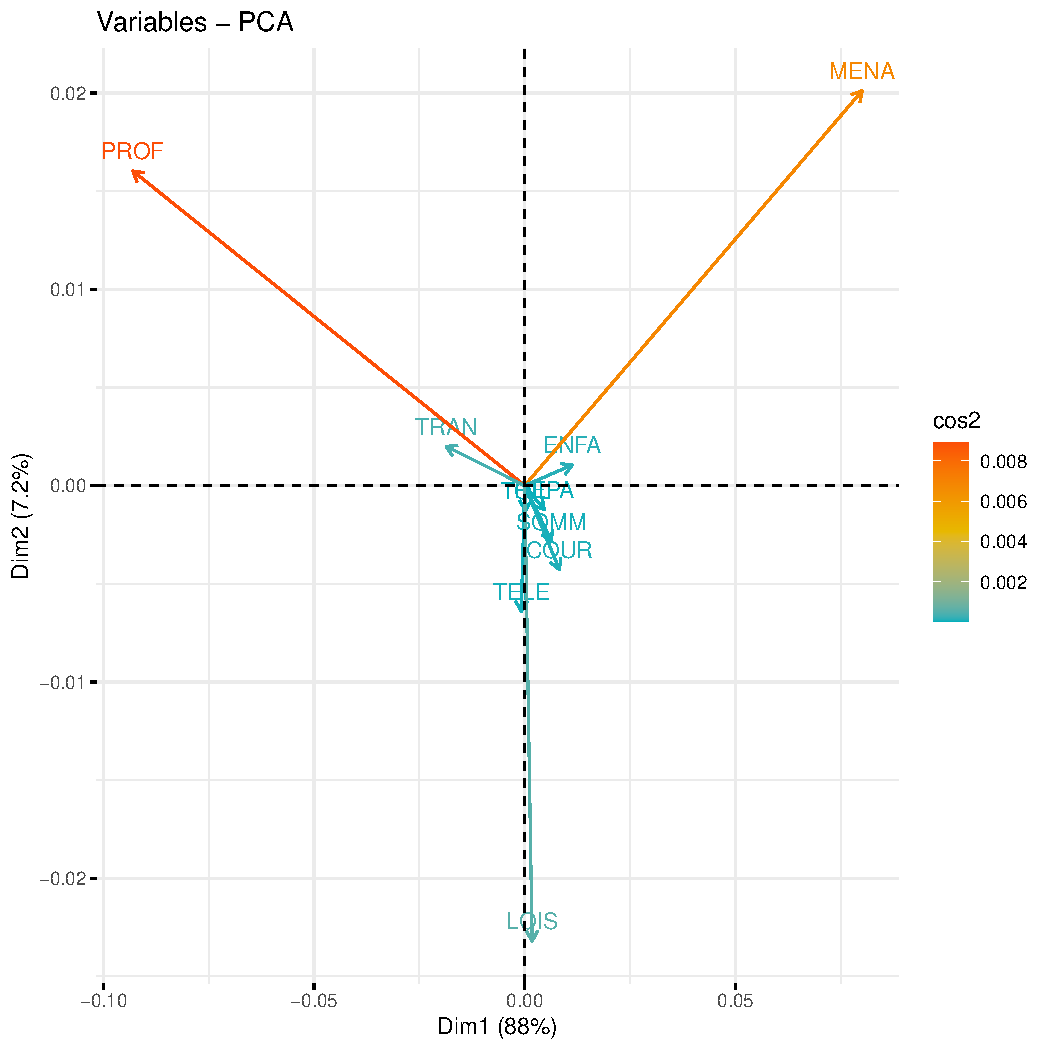
\includegraphics[scale=0.4]{../plot/pca-attribute-projection.pdf}
  \caption{PCA attribute projection}
  \label{fig:pca-attribute-projection}
\end{figure}
\begin{minted}{R}
pdf("plot/pca-instance-projection.pdf")
library("factoextra")
fviz_pca_ind(pca, col.var = "cos2", col.ind = "cos2",
             gradient.cols = c("#00AFBB", "#E7B800", "#FC4E07"))
dev.off()  
\end{minted}
The resulting plot is in figure \ref{fig:pca-instance-projection}.
\begin{figure}[h]
  \centering
  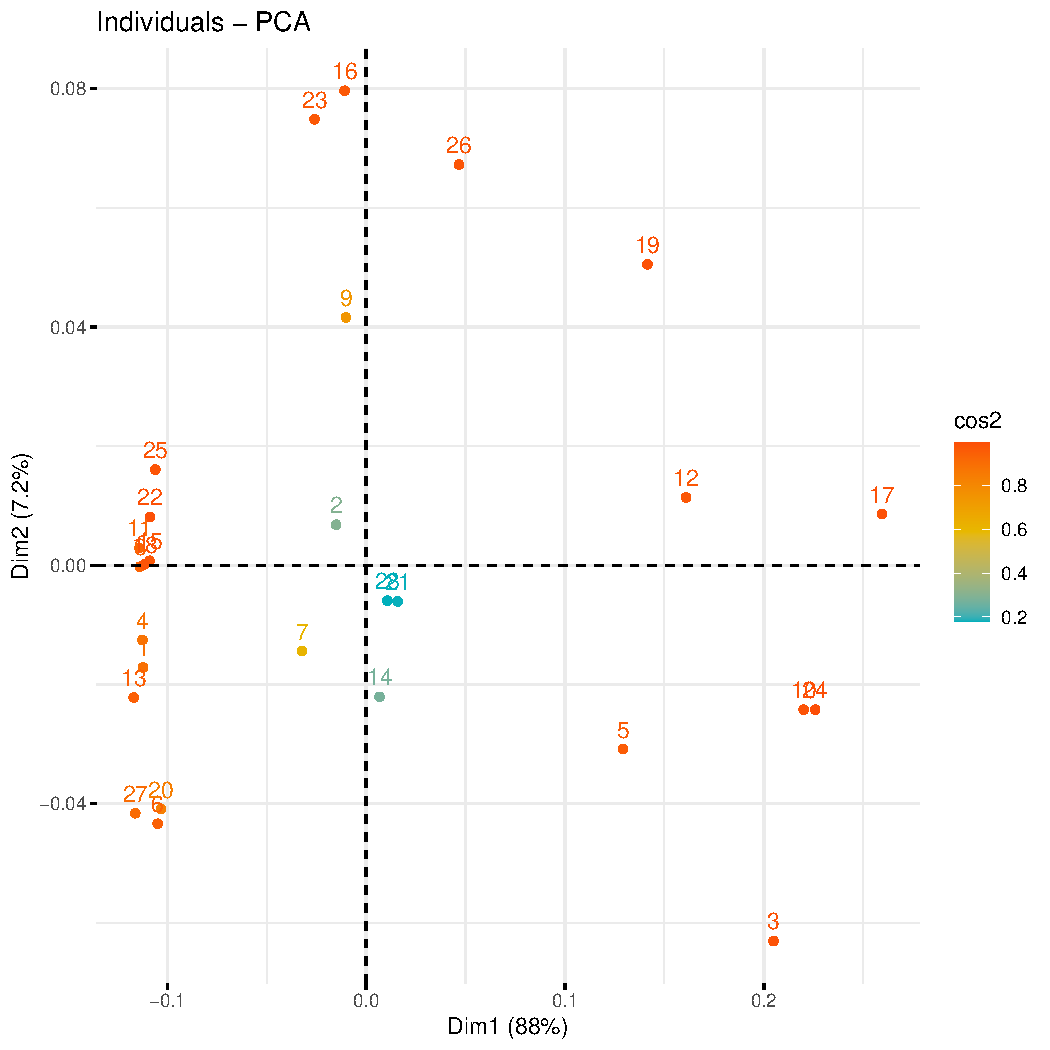
\includegraphics[scale=0.4]{../plot/pca-instance-projection.pdf}
  \caption{PCA instance projection}
  \label{fig:pca-instance-projection}
\end{figure}
As according to the percentages of explained variance we see that most instance
have a good projection quality.
\section{Clustering}
To analyse similarities in between the group profiles themselves we performed
clustered the instances throught the use of the KMeans Machine Learning
algorithm.\par This algorithm first requires to manually set the number of
clusters in which the instances shall be grouped together.
%% \section{Annex}
%% \label{section:annex}
%% \subsection{Carte Radar}
%% \foreach\x in {1, ..., 28}{%
%%   \includegraphics[height=5.4cm]{../plot/radar-chart/radar-chart-\x.pdf}
%% }
%% \subsection{Graphique à barres}
%% \foreach\x in {1, ..., 28}{%
%%   \includegraphics[height=5.4cm]{../plot/bar-plot/bar-plot-\x.pdf}
%% }
\end{document}
